\documentclass[a4paper,12pt]{article}
\usepackage{relsize}
\usepackage[margin=3cm]{geometry} %Definiere Rand
\usepackage{graphicx} % Zum Einbinden von Bildern
\usepackage[english]{babel} % Direkte Eingabe von Umlauten
\usepackage[utf8]{inputenc} % Direkte Eingabe von Umlauten
\usepackage[T1]{fontenc}  % Direkte Eingabe von Umlauten
\usepackage{pgfplots} % Zum Einfuegen von Plots
\pgfplotsset{compat=1.14} % Damit wird beim Plotten keinen Error bekommen
\usepackage[section]{placeins} %Damit Bilder in der Section bleiben
\usepackage{amsmath} % Standard fuer mathematische Ausdruecke
\usepackage{amssymb} % Weitere Symbole
\usepackage{mathtools} % Fuer weitere mathematische Ausdruecke
\usepackage{siunitx} % Um SI-Einheiten anzugeben
\usepackage[font=small,labelfont=bf]{caption} % Kleinerer Text bei Captions
\usepackage{tabu} % Anderes Tabellenenvironment, wird am Ende fuer die Namen verwendet
\usepackage{subcaption} % Side-by-side figures with minipage
\usepackage{url} % Damit man urls zitieren kann
\usepackage[autostyle=true,german=quotes]{csquotes} % Damit Zitieren leichter ist; Bsp: \enquote{nur}
\usepackage[nottoc,numbib]{tocbibind} % Damit die Referenzen im Inhaltsverzeichnis erscheinen
% Die folgenden zwei Zeilen benennen "Inhaltsverzeichnis" zu "Referenzen um
\usepackage{standalone} % Zum Outsourcen von Plots
\addto\captionsngerman{\renewcommand{\bibname}{Referenzen} \renewcommand{\refname}{Referenzen}} % Benennt "Literatur" in "Referenzen" um
\sisetup{range-phrase=-} % Wie SI-Intervalle angezeigt werden
\usepackage{setspace} % Damit die naechsten funktionieren
\renewcommand{\topfraction}{0.85} % Let top 85% of a page contain a figure
\renewcommand{\textfraction}{0.1} % Default amount of minimum text on page (Set to 10%)
\renewcommand{\floatpagefraction}{0.75} % Only place figures by themselves if they take up more than 75% of the page
\DeclareSIPostPower\tothefourth{4} % SI-Einheiten zur 4. Potenz
%
\makeatletter
\newcommand*{\rom}[1]{\expandafter\@slowromancap\romannumeral #1@}
\makeatother %roman numerals
\usepackage{threeparttable, tablefootnote}
\DeclareSIUnit\torr{torr}
\usepackage{circuitikz} %For circuits
\renewcommand{\d}{\mathrm{d}}
\newcommand{\intl}{\int\limits}
\sisetup{math-micro=\text{µ},text-micro=µ}
\usepackage{hyperref} % For hyperlinks to be clickable
\begin{document}
%
    \title{[Title of thesis]\\
    \vspace{2em}
    Bachelorarbeit\\
    \vspace{2em}
    \smaller[2]{}zur Erlangung des akademischen Grades\\
    Bachelor of Science (BSc)\\
    \vspace{2em}
    eingereicht an der\\
    Fakult{\"a}t f{\"u}r Mathematik, Informatik und Physik\\
    der\\
    Leopold-Franzens-Universit{\"a}t Innsbruck\\
    \vspace{1.5em}
    von}

    \author{
 	\LARGE Bernhard Gstrein\\
 	\vspace{.5em} \\
 	Betreuer:\\
 	Univ.Prof. Dr. Helmut Ritsch\\
 	\small Institut f{\"u}r Theoretische Physik\\
 	\vspace{1em}
	}
    
    \date{Innsbruck, 2019}

    \maketitle
   
   \begin{abstract}
	Hier die Kurzfassung in ganzen Sätzen.
	\end{abstract}
   
\newpage
   
\tableofcontents
 
\newpage
    

\section{Atoms in optical cavities}

In cavity quantum electrodynamics (cavity QED) there are cases where the spontaneous emission of the atoms is essential. It's possible, however, to suppress the spontaneous emission if we detune the laser far from the atomic resonance frequency. In that case coherent scattering of the photons are dominant and there's a significant optical dipole force. Due to the confinement of the cavity, the back-action of the atoms onto the laser becomes significant, whereas it's negligible in free space.

\section{Types of optical cavities}
There are different types of cavities, such as the bow-tie, the ring and the Fabry-Perot cavity. In the case of the Fabry-Perot cavity, there are two curved mirrors separated by a distance $d$. If $d = n \lambda / 2$, the system is in resonance and there's a strong light field in the cavity. Thus boundary conditions on light space determine the modes of the frequency space.

\section{The Jaynes-Cummings Hamiltonian}
The Jaynes-Cummings model describes the interaction of a two-level atom with a single mode of a cavity field \cite{jaynes}. The Jaynes-Cummings Hamiltonian is:

\begin{align}
\begin{split}
H_\text{JC} = \underbrace{p^2 / 2m}_\text{atom} + \underbrace{V_\text{ext}(x)}_\text{external potential} - \underbrace{1/2 \hbar \omega_\text{a} \sigma_z}_\text{atomic transitions} - \underbrace{\hbar \omega_\text{c} a^\dagger a}_\text{field} + \underbrace{\hbar \eta (a e^{i \omega_\text{l} t} + a^\dagger e^{-i \omega_\text{l} t})}_\text{pumping} + \\
+ \underbrace{\hbar g_0 \cos(kx) (\sigma^+ a + \sigma^- a^\dagger)}_\text{field-atom interaction},
\end{split}
\end{align}where $\omega_\text{a}$ is the resonance frequency of the atom, $\sigma_z$ the Pauli spin matrix, $\omega_\text{c}$, the resonance frequency of the cavity, $a^\dagger$ and $a$ the creation and annihilation operators, $\eta$ the pumping strength, $\omega_\text{l}$ the frequency of the laser, $U_0$ the coupling constant and $\sigma^+$ and $\sigma^-$ the raising and lowering operators. A detailed derivation of the Jaynes-Cummings Hamiltonian can be found at \cite{collapseandrevival}. In order to get rid of the explicit time-dependence, we transform the Hamiltonian to a frame rotating with $\omega_\text{l}$. The Hamiltonian now reads:

\begin{align}
\begin{split}
H_\text{JC} = \frac{p^2}{2m} + V_\text{ext}(x) - \hbar \Delta_\text{a} \sigma_z - \hbar \Delta_\text{c} a^\dagger a + \hbar \eta (a + a^\dagger) + \\
+ \hbar g_0 \cos(kx) (\sigma^+ a + \sigma^- a^\dagger),
\end{split}
\end{align}where $\Delta_\text{a} = \omega_\text{l} - \omega_\text{a}$ and $\Delta_\text{c} = \omega_\text{l} - \omega_\text{c}$.

\section{Detuning}
In our case, the pumping laser is far detuned from the atomic resonance frequency, i.e. $\Delta_\text{a} = \omega_\text{l} - \omega_\text{a}$ is large. Thus the excitation probability of the atom is vanishing and we neglect the $\sigma_z$-term. Now we derive heuristically a modified Hamiltonian. Going to the Heisenberg picture:

\begin{align}
\dot{a} = \frac{i}{\hbar} [H, a] = i \Delta_\text{c} a - i \eta -i g_0 \cos(kx) \sigma^-.
\end{align}The time-derivative for the raising operator reads:

\begin{align}
\dot{\sigma}^+ = -i \Delta_\text{a} \sigma^+ + i g_0 \cos(kx) a^\dagger.
\end{align}We're not interested in fast dynamics, so we set $\dot{\sigma}^+ = 0$. We obtain

\begin{align}
\sigma^+ = \frac{g_0 \cos(kx)}{\Delta_\text{a}} a^\dagger && \sigma^- = \frac{g_0 \cos(kx)}{\Delta_\text{a}} a.
\end{align}We obtain:

\begin{align}
\dot{a} = -i \Delta_\text{c} a + \frac{i g_0 \cos(kx)}{\Delta_\text{a}} a - i \eta.
\end{align}We can thus make a guess of the effective Hamiltonian:

\begin{align}
H = \frac{p^2}{2m} = V_\text{ext}(x) - \hbar \Delta_\text{c} a^\dagger a + \hbar \eta (a + a^\dagger) + \hbar \frac{g_0^2 \cos(kx)^2}{\Delta_\text{a}}.
\end{align}
\section{Pumped cavity}
The derivation for the Hamiltonians for the following sections is taken from \cite{donner}.

\subsection{Longitudinal Pump}
In the simulation we set the external Potential to 0. We set $U_0 \coloneqq g_0^2/\Delta a$. Since we are working with a red-detuned laser, $\Delta a$ and $\Delta c$ are smaller 0. The Hamiltonian is:

\begin{align}
H_\text{long} = \frac{p^2}{2m} + V_\text{ext}(x) - \hbar \Delta_c a^\dagger a + \hbar \eta (a + a^\dagger) + \hbar U_0 \cos(kx)^2 a^\dagger a.
\end{align}We want to make sure all quantities are expressed with the recoil energy $E_r = \hbar \omega_r$, where $\omega_r = \hbar k^2 / 2m$ is the recoil frequency. Therefore we factor our $E_r$ to see what we have to type into the program:

\begin{align}
\begin{split}
H_\text{long} = \hbar \omega_r \biggl( \frac{1}{\hbar^2 k^2} p^2 + \frac{1}{\hbar \omega_r} V_\text{ext}(x) - \frac{1}{\omega_r} \Delta_c a^\dagger a + \frac{1}{\omega_r} \eta (a + a^\dagger) + \\
 + \frac{1}{\hbar \omega_r} U_0 \cos(kx)^2 a^\dagger a \biggr).
\end{split}
\end{align}In the simulation program, we will thus set $\hbar = 1$ and divide each quantity by the preceding factors.

\subsection{Transversal pump}
Again, in the simulation we set the external potential to 0. Here we only consider one dimension, so we set $z=0$.

\begin{align}
\begin{split}
H_\text{transv} = \frac{p^2}{2m} + V_\text{ext}(x) - \hbar \Delta_c a^\dagger a - \hbar \eta \cos(kx) \cos(kz) (a + a^\dagger) + \\
 + \hbar U_0 \cos(kz)^2 + \hbar U_0 \cos(kz)^2 a^\dagger a.
\end{split}
\end{align}As previously mentioned, keeping the right dimensionality in the simulation is very important.

\section{Results}
The longitudinal spatial wave function densities are depicted in Figure~\ref{long_eta} for different values of $\eta$.

\begin{figure}[htp]
\centering
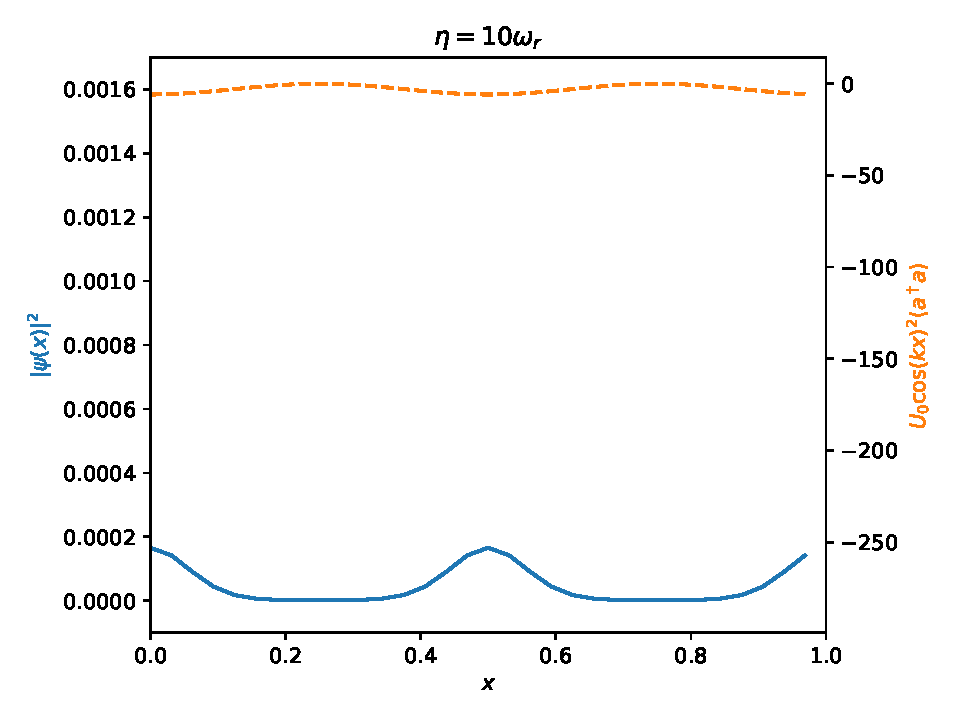
\includegraphics[width=.3\textwidth]{long_eta_10.pdf}\hfill
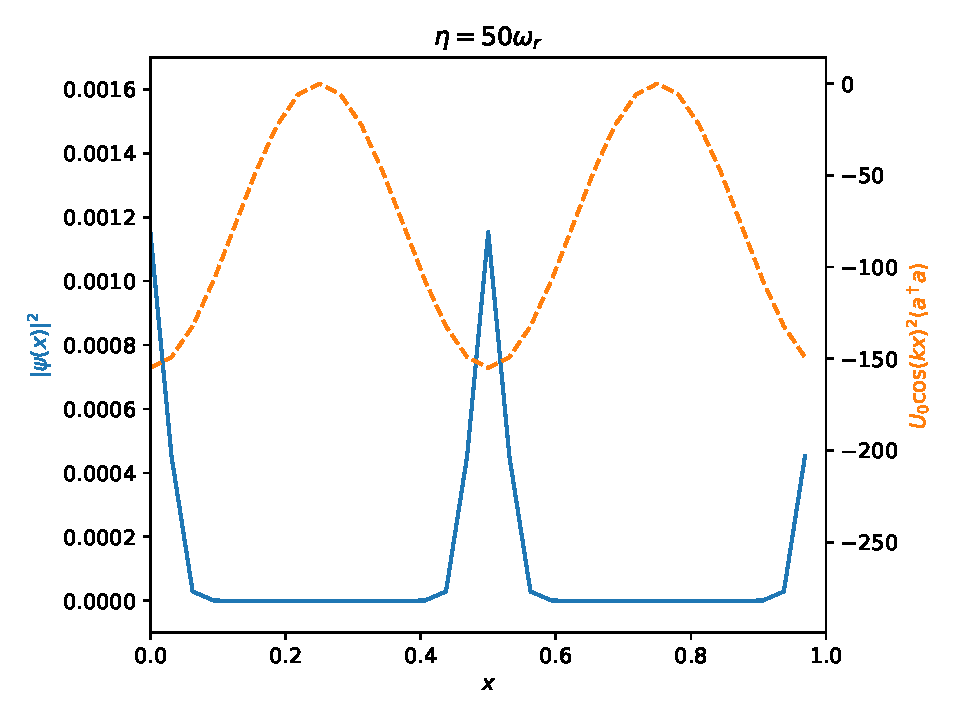
\includegraphics[width=.3\textwidth]{long_eta_50.pdf}\hfill
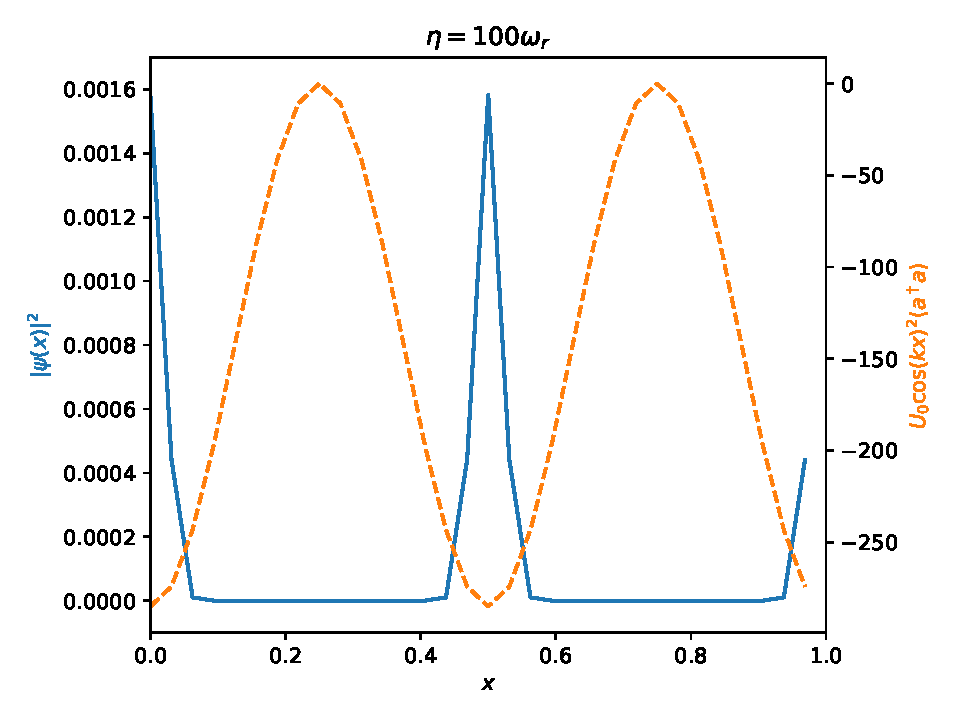
\includegraphics[width=.3\textwidth]{long_eta_100.pdf}
\caption{Longitudinal wave function densities for $\eta = 10 \omega_r$, $\eta = 50 \omega_r$ and $\eta = 100 \omega_r$.}
\label{long_eta}
\end{figure}
\FloatBarrier

\noindent Figures \ref{long_pmp_bunch} and \ref{trans_pmp_bunch} depict the bunching parameter $\langle \cos(kx)^2 \rangle$ each. We did not obtain any meaningful results with the order parameter $\langle \cos(kx) \rangle$.

\begin{figure}[ht]
  \centering
  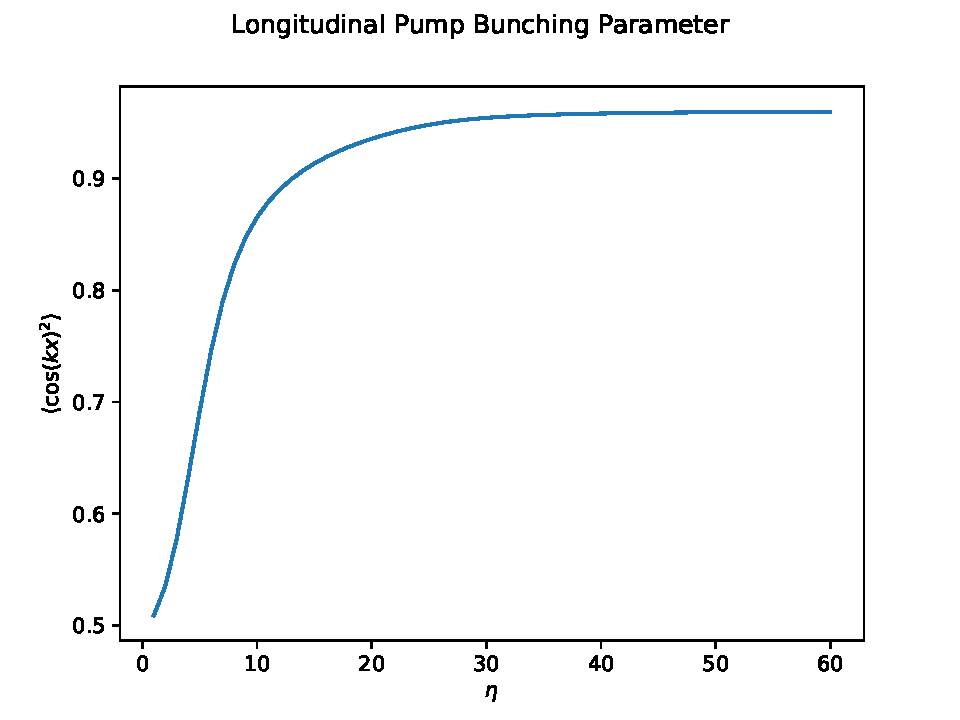
\includegraphics[width=.7\linewidth]{long_pmp_bunch.pdf}
  \caption{Bunching parameter for longitudinal pump with $\Delta_c = -10 \omega_r$ and $U_0 = -1 \omega_r$.}
  \label{long_pmp_bunch}
\end{figure}
\FloatBarrier

\begin{figure}[ht]
  \centering
  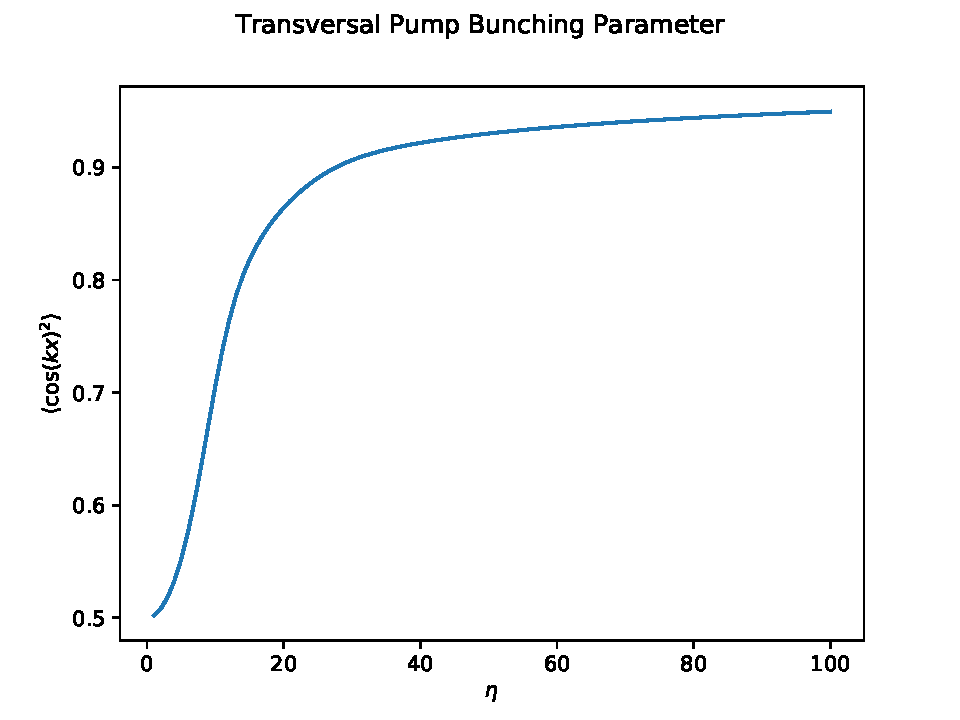
\includegraphics[width=.7\linewidth]{trans_pmp_bunch.pdf}
  \caption{Bunching parameter for transversal pump with $\Delta_c = -10 \omega_r$ and $U_0 = -1 \omega_r$.}
  \label{trans_pmp_bunch}
\end{figure}
\FloatBarrier

\noindent To obtain the order parameter as a function of $\eta$ for transversal pump, we used the mean-field approximation, as depicted in \cite{cold_atoms}. For now, a simple Euler algorithm will do. The results can be seen in Figure~\ref{trans_pmp_order}. Strangely, there is no threshold at which order sets in, but rather a gradual shift. We also tried to tweak the parameters similar to \cite{Nagy2008}, which unfortunately made the wave function all but disappear.

\begin{figure}[ht]
  \centering
  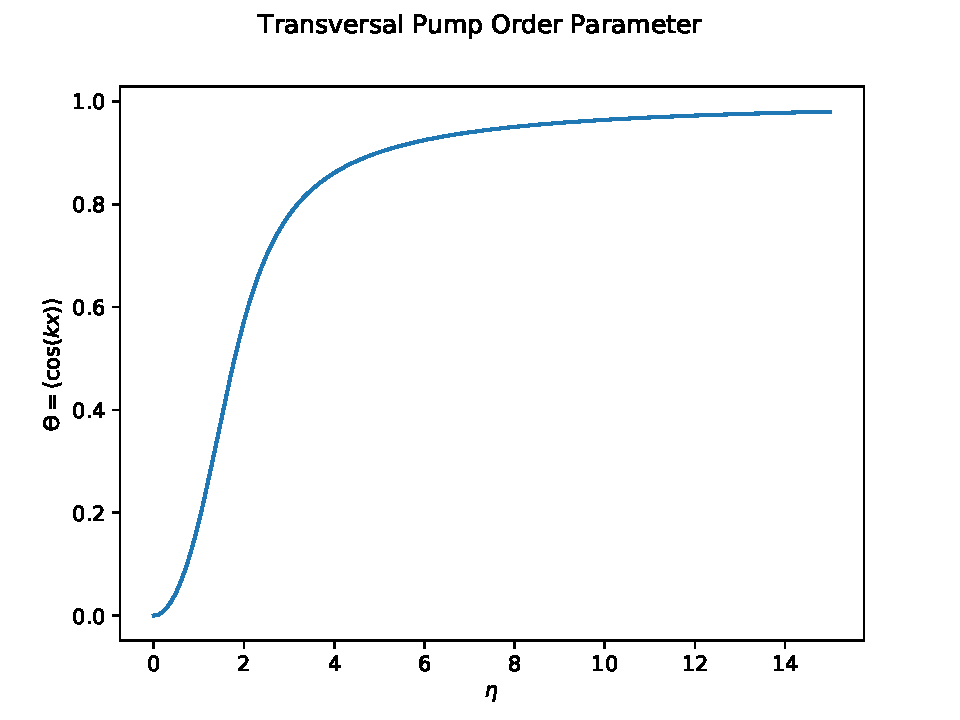
\includegraphics[width=.7\linewidth]{trans_pmp_order.pdf}
  \caption{Order parameter for transversal pump with $\Delta_c = -1 \omega_r$, $U_0 = -1 \omega_r$ and $\kappa = \omega_r$.}
  \label{trans_pmp_order}
\end{figure}
\FloatBarrier


\newpage

\bibliographystyle{unsrt}
\bibliography{bibliography}



\end{document}
